\documentclass[12pt]{article}
\usepackage[spanish]{babel}
\usepackage{multirow}
\usepackage{amstext}
\usepackage{blindtext}
\usepackage{multicol}
\usepackage{array}
\usepackage{booktabs}
\usepackage{varioref}
\usepackage[linktocpage=true]{hyperref}
\usepackage[capitalise,noabbrev]{cleveref}
\usepackage{tocloft}
\usepackage[utf8]{inputenc}
\usepackage[nottoc]{tocbibind}
\usepackage{graphicx}
\usepackage{boxhandler}
\usepackage{caption}
\usepackage{appendix}
\usepackage{mathptmx}
\usepackage{setspace}
\usepackage{ifxetex}
\usepackage{xparse}
\usepackage[indentafter]{titlesec}
\usepackage[style=numeric,language=american,maxnames=4,minnames=3,sortcites=true]{biblatex}
\usepackage{geometry}
\usepackage{csquotes}
\usepackage{longtable}
\usepackage{xcolor}
\usepackage{tcolorbox}
\usepackage{parskip}
\usepackage{subfig}
\usepackage{listings}
\geometry{
  letterpaper,
  left=2.54cm,
  right=2.54cm,
  bottom=2.54cm,
  top=2.54cm,
}

% Definitions
%%%%%% start: define some names here %%%%%%
\newcommand{\longvertspacing}{~\\~\\~\\~\\~\\~\\}
\newcommand{\mylinespacing}{\vspace{1em}}
\newcommand{\myoptpg}{\textbf{THIS PAGE IS OPTIONAL}}
\newcommand{\mytitle}{Optimización de Bajo Costo Adaptable para Recursos
  Computacionales Mediante Computación Distribuida}
\newcommand{\myname}{Nicolas Jaramillo Mayor}
\newcommand{\degreetype}{\capitalize{my degree}}
\newcommand{\mydegree}{\capitalize{my degree name}}
\newcommand{\myprogram}{\capitalize{my program name}}
%%%% choose: May, August, December  %%%%
\newcommand{\mymonth}{Marzo}
\newcommand{\myyear}{2023}
\newcommand{\myadvisor}{John Sanabria}
\newcommand{\committeememberA}{León Escobar}
%%%% Commands %%%%
\renewcommand{\cftsecleader}{\cftdotfill{\cftdotsep}}
\renewcommand{\cftfigleader}{\cftdotfill{\cftdotsep}}
\renewcommand{\cfttableader}{\cftdotfill{\cftdotsep}}
\renewcommand{\cftsecfont}{\normalfont\MakeUppercase}
\renewcommand{\cftsubsecfont}{\normalfont}
\renewcommand{\cftsubsubsecfont}{\normalfont}
\renewcommand{\cftsecpagefont}{\normalfont}
\renewcommand{\cfttabpresnum}{Tabla }
\renewcommand{\cfttabaftersnum}{.\hspace{1ex}}
\renewcommand{\cfttoctitlefont}{\hspace*{\fill}\normalsize\MakeUppercase}
\renewcommand{\cftaftertoctitle}{\hspace*{\fill}}
\renewcommand{\contentsname}{Tabla de Contenido}
\renewcommand{\cftlottitlefont}{\hfill\normalsize\MakeUppercase}
\renewcommand{\cftafterlottitle}{\hfill}
\renewcommand{\cftloftitlefont}{\hfill\normalsize\MakeUppercase}
\renewcommand{\cftafterloftitle}{\hfill}
\setlength{\cftparskip}{2ex}
\setlength{\cftfignumwidth}{10.5ex}
\setlength{\cfttabnumwidth}{8ex}
\setlength{\cftfigindent}{0ex}
\setlength{\cfttabindent}{0ex}
\setlength{\columnsep}{1cm}
\makeatletter
\let\latexl@section\l@section{}
\def\l@section#1#2{\begingroup\let\numberline\@gobble\latexl@section{#1}{#2}\endgroup}
\let\latexl@subsection\l@subsection{}
\def\l@subsection#1#2{\begingroup\let\numberline\@gobble\latexl@subsection{#1}{#2}\endgroup}
\let\latexl@subsubsection\l@subsubsection{}
\def\l@subsubsection#1#2{\begingroup\let\numberline\@gobble\latexl@subsubsection{#1}{#2}\endgroup}
\makeatother
%% set figure path
\graphicspath{{figures/}}
%% captions
\captionsetup{labelsep=period, justification=raggedright,
  singlelinecheck=false}
%% biblatex
\DeclareLanguageMapping{american}{american-apa}
\addbibresource{ref.bib}
%% set fontsize
\fontsize{12}{1} \selectfont
\singlespacing{}
%\usepackage{indentfirst}
\setlength{\parindent}{6.5ex}

%%%% heading 1
\titleformat{\section}
{\normalsize\center}
{}
{0pt}
{\MakeUppercase}
%%%% heading 2
\titleformat{\subsection}
{\normalsize\bf}
{}
{0pt}
{\capitalize}
%%%% heading 3
\titleformat{\subsubsection}
{\normalsize\bf}
{}
{0pt}
{\capitalize}
%%%% heading 4
\titleformat{\paragraph}
{\normalsize\bf\itshape}
{}
{0pt}
{\capitalize}
%\titleformat{⟨command⟩}[⟨shape⟩]{⟨format⟩}{⟨label⟩}{⟨sep⟩}{⟨before-code⟩}[⟨after-code⟩]

%% a new center environment
\newenvironment{tightcenter}{%
  \setlength\topsep{0pt}
  \setlength\parskip{0pt}
  \begin{center}
    }{%
  \end{center}
}
%% adjust quotation environment margin
\renewenvironment{quote}{%
  \list{}{%
    \leftmargin0cm   % this is the adjusting screw
    \rightmargin\leftmargin{}
  }
  \item\relax
}
{\endlist}

%%%%%% capitalize from stackexchange %%%%%% 
\ExplSyntaxOn{}
\NewDocumentCommand{\capitalize}{>{\SplitList{~}}m}
{
  \seq_clear:N \l_capitalize_words_seq
  \ProcessList{#1}{\CapitalizeFirst}
  \seq_use:Nn \l_capitalize_words_seq {~}
}
\NewDocumentCommand{\CapitalizeFirst}{m}
{
  \capitalize_word:n { #1 }
}

\sys_if_engine_pdftex:TF
{
  \cs_set_eq:Nc \capitalize_tl_set:Nn { protected@edef }
}
{
  \cs_set_eq:NN \capitalize_tl_set:Nn \tl_set:Nn
}

\cs_new_protected:Nn \capitalize_word:n
{
  \capitalize_tl_set:Nn \l_capitalize_word_tl { #1 }
  \seq_if_in:NfTF \g_capitalize_exceptions_seq { \tl_to_str:n { #1 } }
  % exception word
  { \seq_put_right:Nn \l_capitalize_words_seq { #1 } }
  % exception word
  % to be uppercased
  { \seq_put_right:Nx \l_capitalize_words_seq { \tl_mixed_case:V
      \l_capitalize_word_tl } }
}
\cs_generate_variant:Nn \tl_mixed_case:n { V }
\NewDocumentCommand{\AppendToList}{m}
{
  \clist_map_inline:nn { #1 }
  {
    \seq_gput_right:Nx \g_capitalize_exceptions_seq { \tl_to_str:n { ##1 } }
  }
}
\cs_generate_variant:Nn \seq_if_in:NnTF { Nf }
\seq_new:N \l_capitalize_words_seq
\seq_new:N \g_capitalize_exceptions_seq
\ExplSyntaxOff{}

\AppendToList{a,is,of,óf}
%%%%%% capitalize from stackexchange %%%%%% 

\title{\MakeUppercase{\normalsize\mytitle}\vspace{-2em}}
\author{\vspace{-5ex}}
\date{\vspace{-5ex}}

\begin{document}
\onehalfspacing

\maketitle

%% roman for frontmatter
\pagenumbering{roman}
\thispagestyle{empty}
\longvertspacing{}
\begin{tightcenter}
  por
\end{tightcenter}
\mylinespacing{}
\begin{tightcenter}
  \myname{}
\end{tightcenter}
{~\\~\\~\\~\\}
%\longvertspacing{}
\begin{tightcenter}
  Una tesis presentada para la obtención del grado de \degreetype\\
  en la Facultad de \myprogram~de la  \\
  Universidad del Valle
\end{tightcenter}
\mylinespacing{}
\begin{tightcenter}
  \mymonth~\myyear{}
\end{tightcenter}
\mylinespacing{}
\begin{tightcenter}
  Director de tesis, \myadvisor{}
\end{tightcenter}
\begin{tightcenter}
  Co-director de tesis, \committeememberA{}
\end{tightcenter}
\vspace{8mm}
\begin{tightcenter}
  \begin{minipage}{0.11\textwidth}
    % Picture
    
\includegraphics[width=\textwidth]{uv.png}
  \end{minipage}
\end{tightcenter}
%% copyright page %%

\pagenumbering{arabic}
\setcounter{page}{2}

%% abs page %%
\begin{spacing}{1.5}
  \begin{tightcenter}
    \section{Agradecimientos}
    \mylinespacing
  \end{tightcenter}

  Quiero expresar mi más profundo agradecimiento a Valentina Salamanca, quien ha sido una figura fundamental en el desarrollo de esta tesis. Su apoyo, compañía y consejos han sido invaluables en todo el proceso. Siempre estuvo dispuesta a brindar su ayuda y apoyo, incluso en los momentos más difíciles, lo que me permitió completar este trabajo de investigación de manera exitosa.

  Valentina, quiero que sepas que tu influencia positiva en mi vida y en mi carrera será recordada siempre. Sin tu ayuda y apoyo, no habría sido posible completar este proyecto de investigación con éxito. Tu contribución ha sido fundamental para mi crecimiento personal y profesional, y estoy profundamente agradecido por todo lo que has hecho por mí. ¡Gracias!

  Me gustaría expresar mi profunda gratitud a John Sanabria y León Escobar, quienes fueron mis tutores durante el desarrollo de esta tesis. Su paciencia y dedicación hicieron posible que pudiera concluir este proyecto de investigación de manera exitosa. Su guía y sabiduría fueron invaluables para mí, y estoy muy agradecido por su ayuda y apoyo.

  Quiero expresar mi agradecimiento al profesor Stevens Paz por su dedicación y apoyo durante el desarrollo de mi tesis. Su ayuda y opiniones fueron invaluables para mí, y estoy muy agradecido por su apoyo constante.

  Quiero agradecer a mis padres por su apoyo incondicional durante todo el proceso de desarrollo de esta tesis. Su amor y su apoyo han sido fundamentales para mi éxito, y estoy profundamente agradecido por todo lo que han hecho por mí. Estoy muy agradecido por su dedicación y apoyo constante. Muchas gracias, mamá y papá, por todo lo que han hecho por mí. Les quiero mucho.

  Quiero aprovechar este momento para expresar mi más sincero agradecimiento a mis queridos amigos Juan José Dorado, Sara Maradiago, Gina Parra, Melissa Gonzáles, Michelle Gonzáles y Alejandro Caicedo. Su inquebrantable amistad y apoyo durante este largo y desafiante camino de mi tesis ha sido invaluable.

  Desde el principio, estuvieron a mi lado, brindándome ánimo y aliento cuando más lo necesitaba. Sus palabras y motivación me impulsaron a seguir adelante incluso en los momentos más difíciles. Su presencia constante en mi vida ha sido un recordatorio de que no estoy solo en este viaje.

  Agradezco también su disposición constante para escuchar mis preocupaciones y brindar soluciones creativas a los desafíos que se presentaron en el camino. Su empatía y paciencia me ayudaron a superar obstáculos y encontrar soluciones cuando las cosas se volvían complicadas.

  No puedo expresar suficientemente cuánto significa para mí tener amigos tan maravillosos como ustedes. Su apoyo incondicional y su amistad duradera son tesoros que valoraré por siempre.

  A medida que culmina esta etapa de mi vida académica, quiero que sepan que su influencia positiva ha dejado una huella profunda en mí. No solo han sido amigos increíbles, sino que han sido pilares fundamentales en mi crecimiento personal y académico.

  Otros agradecimientos:

  Carlos Tovar, Michelle Sanchez, Cristina Rios, Santiago Duque y Santiago García.

  \mylinespacing
  \mylinespacing
  \begin{tightcenter}
  \end{tightcenter}
\end{spacing}
\begin{spacing}{1.5}
  \begin{abstract}
    El presente trabajo tiene como objetivo proponer una metodología para aprovechar al máximo los recursos computacionales subutilizados en el clúster Bochica y la sala de computación Jürgen Tischer del departamento de Matemáticas de la Universidad del Valle. Se propone la implementación de un sistema distribuido con un gestor de cola de tareas y capacidades de paralelización para lograr una mayor eficiencia en investigaciones matemáticas. Se investiga y se propone una implementación específica del sistema distribuido y se evalúa su rendimiento y eficiencia. Los resultados obtenidos muestran una mejora significativa en el poder máximo de cómputo obtenible por el sistema con respecto a un sistema no distribuido, lo que resultará beneficioso para el entorno académico e investigativo de la Universidad del Valle. Este trabajo contribuye al campo de la informática y la matemática aplicada, al mejorar el aprovechamiento de los recursos computacionales en entornos académicos.
  \end{abstract}
\end{spacing}
%% content lists %%
\setcounter{tocdepth}{3} % can change 2 for heading 2
\tableofcontents
\newpage
\listoftables
\newpage
\listoffigures

\begin{doublespace}
\begin{tightcenter}
\section{1. Introducción}
\mylinespacing
\end{tightcenter}

La avanzada época de la computación nos ha llevado a un presente donde las necesidades de procesamiento crecen constantemente, especialmente en el campo de la investigación, donde cada día se requiere más que solo teoría. Aún así en la Universidad del Valle no existen, de forma accesible, medios con los que ejecutar trabajos con requerimientos computacionales extensos.

\vspace{3mm} 

En nuestra alma mater existen recursos computacionales subutilizados, los cuales podrían ser aprovechados para crear un servicio computacional con gran poder de procesamiento dispuesto para cálculos con fines académicos. Esto resultaría de gran utilidad para la comunidad universitaria, ya que permitiría la realización de nuevos trabajos investigativos que actualmente no son posibles por la carencia de un medio con estas capacidades.

\vspace{3mm} 

Estos recursos son los computadores de la Sala \textit{Jürgen Tischer}, elementos normalmente inutilizados en los periodos en los que no hay clase y el clúster computacional \textit{Bochica}, actualmente en desuso. Ambos bienes pertenecen al Departamento de Matemáticas de la Universidad del Valle.

\vspace{3mm} 

Este proyecto propone integrarlos e implementar un gestor de cola de tareas con capacidades de procesamiento paralelo y distribuido. De esta manera sería posible alcanzar una mayor capacidad de procesamiento y a su vez, facilitar su uso apropiado para la investigación y la docencia.


\mylinespacing
\mylinespacing
\begin{tightcenter}
\end{tightcenter}
\end{doublespace}

\begin{spacing}{1.5}
  \begin{tightcenter}
    \section{2. Análisis de recursos y necesidades}
    \label{chap:recursos-necesidades}
    \mylinespacing
  \end{tightcenter}

  En este capítulo se hace un análisis detallado de los recursos informáticos disponibles para esta tesis en el Departamento de Matemáticas de la Universidad del Valle.

  \subsubsection{2.1 Recursos computacionales}
  El departamento de Matemáticas cuenta con dos espacios dedicados a la utilización de recursos computacionales: un clúster computacional, conocido como Clúster Bochica y una sala de cómputo llamada Sala de Cómputo Jürgen Tischer.

  En la siguiente tabla se muestran los computadores y servidores con los que cuentan dichos espacios:
  \vspace{3mm}

  \begin{table}[h!]
    \centering
    \begin{tabular}{p{5cm}|c|c|c}
      \hline
      \textbf{Rubro}                                          & \textbf{Núcleos por Unidad} & \textbf{Unidades} &
      \textbf{Total Núcleos}                                                                                                   \\ \hline
      \textbf{Servidores en Clúster Bochica}                  &                             &                   &              \\ \hline
      COMPUTADOR HP DL360E GEN 8                              & 16                          & 4                 & 64           \\ \hline
      SERVIDOR DELL POWEREDGE 1950                            & 8                           & 4                 & 32           \\ \hline
      \textbf{Subtotal}                                       &                             & \textbf{8}        & \textbf{96}  \\ \hline
      \textbf{Computadores en Sala de Cómputo Jürgen Tischer} &                             &                   &              \\ \hline
      COMPUTADOR WORKSTATION HP Z1                            & 10                          & 2                 & 20           \\ \hline
      COMPUTADOR WORKSTATION HP Z2                            & 8                           & 1                 & 8            \\ \hline
      COMPUTADOR DELL PRECISION T3610                         & 4                           & 30                & 120          \\ \hline
      COMPUTADOR DELL PRECISION T5500                         & 2                           & 7                 & 14           \\ \hline
      \textbf{Subtotal}                                       &                             & \textbf{40}       & \textbf{162} \\ \hline
      \textbf{Total}                                          & \textbf{ }                  & \textbf{48}       & \textbf{258} \\ \hline
    \end{tabular}
    \caption{Recursos Computacionales}
    \label{table:table1}
  \end{table}

  Adicionalmente, los equipos cuentan con unidades de alimentación ininterrumpida (UPS, por sus siglas en inglés), a la par de un dispositivo de conmutación de red (switch) que interconecta a los servidores presentes en el Clúster. Es importante destacar que todos los equipos informáticos mantienen una conexión con la red universitaria perteneciente al campus y, asimismo, disponen de acceso a internet.

  \subsubsection{2.2 Recursos de software}

  La Universidad del Valle dispone de licencias de software que pueden resultar de gran utilidad para el desarrollo de esta tesis, entre ellas se encuentran Wolfram Mathematica, Mathematica Licence Manager, gridMathematica, MATLAB, MATLAB Licence Manager y MATLAB Parallel Server. Además de esto se utilizarán licencias de software de uso libre.

  \subsubsection{2.3 Necesidades por parte del departamento de Matemáticas}

  El profesor León Escobar, quien está a cargo de la sala de Matemáticas Jürgen Tischer y es co-director de esta tesis, ha destacado ciertas características que deben ser tomadas en cuenta en el desarrollo de esta tesis. Entre los principales aspectos destacados se encuentra la oportunidad de emplear computación paralela, utilizando diferentes lenguajes y herramientas como Python, C++, R, Wolfram Mathematica y MATLAB. 

  Además, el profesor ha mencionado que prefiere el uso de Slurm como gestor de cola de tareas, ya que es ampliamente conocido en el ámbito académico y familiar para él.

  \mylinespacing
  \mylinespacing
  \begin{tightcenter}
  \end{tightcenter}
\end{spacing}
\begin{spacing}{1.5}
  \begin{tightcenter}
    \section{3. Diseño y metodología}
    \mylinespacing
  \end{tightcenter}

  En este capítulo se describen los métodos utilizados para el diseño y desarrollo del servicio de computación, así como el plan para su implementación.

  \subsection{3.1 Resultados esperados}

  En la siguiente tabla se muestran los logros proyectados para cada uno de los objetivos específicos estipulados en el marco de la tesis.

  \begin{table}[h]
    \centering
    \begin{tabular}{p{7cm}|p{7cm}}
      \hline
      \textbf{Objetivos Específicos}                                 & \textbf{Resultado(s) Esperados}                                          \\
      \hline
      Identificar recursos disponibles y necesidades investigativas. &
      Documento expresando la arquitectura de los recursos y las necesidades a
      considerar. (Este objetivo se desarrolla durante el capítulo \nameref{chap:recursos-necesidades})                                         \\
      \hline
      Diseñar una solución que considere los requerimientos de los usuarios y
      aproveche las capacidades de los recursos computacionales mediante la
      implementación de un gestor de cola de tareas.                 & Documentación, scripts,
      programas y/o pruebas básicas de operación que simplifiquen o automaticen el
      mantenimiento y administración del gestor de cola de tareas.       (Este objetivo se desarrolla durante el capítulo \nameref{chap:3.2})   \\
      \hline
      Llevar a cabo la instalación, documentación y puesta a punto de
      herramientas que apoyen los procesos de investigación y docencia en el área de
      matemáticas, facilitando el uso del servicio.                  & Documentación, scripts y
      programas que automaticen y faciliten la utilización del servicio para los
      estudiantes o profesores. (Este objetivo se desarrolla durante el capítulo \nameref{chap:4.3})                                            \\
      \hline
      Llevar a cabo pruebas de uso de la infraestructura y de las
      aplicaciones desplegadas en este trabajo.                      & Reporte de pruebas en donde se
      evidencie la correcta funcionalidad y la eficiencia de los recursos. (Este objetivo se desarrolla durante el capítulo \nameref{chap:4.4}) \\
      \hline
    \end{tabular}
    \caption{Resultados Esperados}
    \label{table:table2}
  \end{table}

  \subsection{3.2 Tecnologías y aprovechamiento de espacios}
  \label{chap:3.2}
  En esta sección se presentan las diversas especificaciones tecnológicas
  seleccionadas para el proyecto en cuestión.

  \subsubsection{3.2.1 Sistema operativo}
  El sistema operativo utilizado para la instalación de los equipos en este
  proyecto es Rocky Linux.

  \textbf{¿Qué es Rock Linux?}

  Rocky Linux es una distribución de Linux que se basa en el código fuente de
  Red Hat Enterprise Linux (RHEL), el cual se compila y se distribuye de forma
  gratuita y de código abierto. Rocky Linux está diseñado para ser compatible con
  el mismo software, herramientas y aplicaciones que RHEL, y ofrece una
  alternativa de código abierto para los usuarios que anteriormente utilizaban
  CentOS. Lo cual resulta en una herramienta poderosa por la gran cantidad de
  software disponible para los entornos RHEL.

  Este tipo de distribución tipo enterprise está diseñada para ofrecer
  estabilidad y confiabilidad en entornos de producción. La distribución incluye
  una variedad de herramientas y utilidades que facilitan la gestión y el
  mantenimiento de sistemas informáticos, incluyendo servidores y estaciones de
  trabajo. Además, Rocky Linux es compatible con paquetes de software de
  terceros. \cite{RL-1}

  \textbf{Rocky Linux 9}

  La versión específica del software utilizado es Rocky Linux 9 (*complete
  iso o DVD iso*) \cite{RL9-download-1} \cite{RL9-release-1}
  \cite{RHEL-release-1}

  Rocky Linux 9 ofrece soporte para actualizaciones de seguridad de este
  software hasta el 31 de Mayo de 2032 \cite{RL9-EOL-1}. Debido su estabilidad y
  largo ciclo de vida que ofrece, es ideal para minimizar las actualizaciones
  manuales a versiones mayores, lo que simplifica el mantenimiento requerido en
  el largo plazo.

  \textbf{Kernel}

  El kernel o núcleo es la parte central de un sistema operativo. Es el
  componente que se encarga de controlar el hardware y los recursos del sistema.
  El kernel es responsable de administrar la memoria del sistema, asignando y
  liberando recursos de manera eficiente. También se encarga de administrar los
  procesos y subprocesos del sistema, lo que permite que múltiples programas se
  ejecuten al mismo tiempo.

  El kernel es esencial para el funcionamiento del sistema operativo y
  proporciona una capa de abstracción entre el hardware y el software.
  \cite{RHEL-kernel-1}

  El kernel incluido en Rocky Linux 9 es la versión 5.14 LTS, que es bastante
  reciente. Esto significa que tanto los ordenadores antiguos, así como los más
  nuevos en la sala de cómputo pueden beneficiarse de esta actualización, y
  aquellos que se planeen comprar en el futuro cercano también podrán
  aprovecharla. \cite{RL9-release-1}

  \subsubsection{3.2.2 Sistema de Archivos}

  \textbf{XFS}

  Rocky Linux, al igual que RHEL utiliza por defecto XFS como sistema de
  archivos. XFS es un sistema de archivos de alto rendimiento que se utiliza en
  sistemas operativos Linux. Fue desarrollado por Silicon Graphics en la década
  de 1990 y se ha incorporado en el kernel de Linux desde la versión 2.4.

  XFS está diseñado para manejar grandes volúmenes de datos y archivos.
  Algunas de las características de XFS incluyen:

  \begin{itemize}
    \item Alta capacidad de lectura y escritura de archivos.
    \item Sistema de administración de archivos de registro que permite una
          recuperación rápida después de un fallo del sistema.
    \item Sistema de cuotas de disco para limitar el uso de espacio en
          disco por usuario o grupo.
  \end{itemize}

  XFS es una buena opción para sistemas que manejan grandes cantidades de
  datos y aplicaciones que requieren una alta capacidad de lectura y escritura de
  archivos. \cite{RHEL-XFS-1}

  \textbf{NFS}

  NFS (Network File System) es un protocolo de red de alto rendimiento y
  eficiente que permite a los sistemas informáticos compartir archivos y recursos
  a través de una red. Está diseñado para reducir la carga en la red y en el
  servidor. El protocolo utiliza una caché para reducir la cantidad de
  solicitudes de red y aumentar la velocidad de acceso a los recursos
  compartidos. Además, soporta la transferencia de datos en modo ráfaga, lo que
  permite que los datos se transfieran en grandes bloques en lugar de pequeños
  paquetes, lo que aumenta la eficiencia de la transferencia de datos. Es un
  estándar para compartir archivos en sistemas operativos basados en Unix y
  Linux.

  NFS se basa en el modelo cliente-servidor, donde un servidor exporta un
  sistema de archivos o un directorio a través de la red, y los clientes pueden
  montar este sistema de directorio en sus propios sistemas, lo que les permite
  acceder a los archivos y recursos compartidos como si estuvieran en su propia
  máquina.

  El protocolo NFS utiliza un sistema de autenticación y autorización para
  controlar el acceso a los recursos compartidos. Los clientes deben autenticarse
  con el servidor antes de acceder a los recursos compartidos, y el servidor
  puede configurar los permisos de acceso en base a las credenciales de los
  usuarios. \cite{RHEL-NFS-1} \cite{RHEL-NFS-2}

  \subsubsection{3.2.3 Distribución de Aplicaciones}
  Existen diversas opciones para la instalación de aplicaciones en Rocky
  Linux. Una de las formas más comunes es a través del uso de gestores de
  paquetes, como DNF, que permiten descargar e instalar software desde
  repositorios compatibles. Además, también es posible utilizar Flatpak, que
  ofrece una mayor flexibilidad en cuanto a la selección de versiones de
  aplicaciones y resolución de dependencias. Otra opción es mediante el uso de
  Podman, una alternativa más segura a Docker, aunque esta alternativa puede
  resultar más compleja y no es recomendada para usuarios inexpertos.

  En nuestro caso se planificó el uso de Flatpak con Flathub como medio
  principal para la instalación de aplicaciones, debido a que se ejecuta en un
  ambiente encapsulado, evitando así conflictos con las dependencias del sistema.
  Las aplicaciones o librerías que no se pueden obtener de Flathub se instalan
  mediante distintos repositorios.

  \textbf{Repositorios}

  Rocky Linux de base solo cuenta con sus propios repositorios de software,
  lo que acarrea un problema en la insuficiente variedad de programas y
  herramientas. Sin embargo, también existen otros repositorios compatibles
  populares como EPEL (Extra Packages for Enterprise Linux), que proporciona
  software adicional para sistemas basados en Red Hat Enterprise Linux, y RPM
  Fusion, que ofrece una gran cantidad de paquetes de software de código abierto
  que no están disponibles en los repositorios oficiales de la distribución. Al
  tener acceso a estos repositorios, se puede disfrutar de una selección de
  software y herramientas más completa. \cite{RL-repo-1} \cite{RHEL-EPEL-1}
  \cite{rpmfusion-1}

  \textbf{Flatpak}

  Flatpak es un sistema de paquetes de software que permite la distribución
  de aplicaciones de forma independiente de la distribución de Linux. Esto
  significa que los usuarios de Linux pueden descargar e instalar aplicaciones de
  una tienda centralizada (Flathub) sin preocuparse por las diferencias en la
  distribución de Linux que estén utilizando.

  Además, Flatpak se basa en contenedores, lo que significa que las
  aplicaciones y todas sus dependencias se empaquetan en un contenedor aislado.
  Esto permite a las aplicaciones ejecutarse de forma independiente de otras
  aplicaciones y bibliotecas del sistema, lo que ayuda a garantizar la
  estabilidad y la seguridad.

  También existe una tienda centralizada donde los usuarios pueden descargar
  e instalar aplicaciones. La tienda se llama Flathub, es un lugar con una amplia
  selección de software disponible sin costo alguno.

  La mayor ventaja de Flatpak y la razón por la que se escoge como método
  principal para instalar aplicaciones en el sistema es debido al aislamiento de
  dependencias, lo que evita conflictos con el sistema operativo. \cite{FLAT-1}
  \cite{FLAT-2} \cite{RHEL-FLAT-1} \cite{PHOENIX-FLAT-1}

  \textbf{Podman}

  Aunque se proveen las librerías y aplicaciones más comunes en la
  configuración que se realizó, con los distintos repositorios mencionados y el
  uso de flatpaks, hay usuarios que podrían tener aún más necesidades y más
  específicas, por lo que también se tiene Podman como soporte para usuarios
  avanzados.

  Podman es una herramienta de administración de contenedores para Linux.
  Permite a los usuarios crear, ejecutar y gestionar contenedores de manera
  similar a otras herramientas populares, como Docker. Sin embargo, a diferencia
  de Docker, Podman no requiere un servicio del sistema para ejecutar los
  contenedores, lo que significa que estos se ejecutan como procesos normales del
  usuario y pueden administrarse utilizando herramientas y comandos. Además,
  Podman utiliza el concepto de 'pods' en lugar de 'servicios', lo que permite a
  los usuarios agrupar y gestionar varios contenedores relacionados juntos en una
  única entidad lógica.

  Podman es una herramienta de código abierto y se desarrolla como parte del
  proyecto de código abierto de la comunidad de Red Hat. \cite{RHEL-podman-1}

  \subsubsection{3.2.4 Sala de cómputo Jürgen Tischer}

  La sala de cómputo es un lugar principalmente utilizado para impartir clases, pero también podría ser utilizada en los espacios libres para llevar a cabo tareas de cómputo distribuido. Es importante tener en cuenta que, debido a que la sala de cómputo es un espacio compartido, es necesario coordinar con los demás usuarios para evitar conflictos y asegurarse de que todos tengan acceso al equipo y los recursos necesarios.

  \textbf{Wolfram Mathematica}

  En el marco de este proyecto, se llevará a cabo una utilización efectiva de
  las licencias que actualmente se encuentran disponibles en la universidad. Se
  han identificado diversas herramientas y software matemáticos que son de gran
  utilidad para la realización de diversas tareas en el ámbito académico y
  científico, y la universidad cuenta con licencias para tres de ellas: Wolfram
  Mathematica, gridMathematica y MathLM.

  Estas licencias representan una valiosa oportunidad para la comunidad
  universitaria de utilizar herramientas de alta calidad y prestigio en el campo
  de las matemáticas, lo que permitirá mejorar el desarrollo de investigaciones,
  proyectos y actividades en general.

  Wolfram Mathematica es un sistema de software de álgebra computacional
  utilizado en matemáticas, física, ingeniería, ciencias sociales y otros campos.
  Ofrece una amplia gama de capacidades que incluyen análisis simbólico y
  numérico, visualización de datos, programación, modelado de sistemas y más.
  \cite{Wolfram-mathematica-1}

  MathLM es una herramienta de licencia de red de Mathematica que permite a
  las instituciones controlar y administrar el acceso de los usuarios al
  software. Con MathLM, las organizaciones pueden asignar licencias a usuarios
  individuales o grupos de usuarios, lo que les permite acceder al software desde
  cualquier lugar de la red. \cite{Wolfram-mathlm-1}

  gridMathematica es una herramienta de computación distribuida que permite a
  las instituciones y organizaciones compartir la carga de procesamiento de
  Mathematica en múltiples computadoras. Al distribuir el procesamiento de
  cálculos complejos en múltiples sistemas, gridMathematica puede reducir
  significativamente el tiempo necesario para realizar análisis complejos y
  simulaciones. También proporciona un mecanismo para administrar recursos
  computacionales y asegurar que las tareas se distribuyan de manera eficiente.
  Wolfram gridMathematica es una extensión de las capacidades de paralelización
  integradas de Mathematica que ejecuta más tareas en paralelo, en más CPUs y
  GPUs, para una ejecución más rápida. Automatiza la coordinación y gestión de
  procesos sin necesidad de cambios en el código. \cite{Wolfram-grid-1}

  \subsubsection{3.2.5 Clúster Bochica}

  El clúster Bochica es un espacio que cuenta con recursos informáticos, los cuales se planean aprovechar en el marco de esta tesis para llevar a cabo tareas de cómputo general y distribuido. Es importante destacar que, debido a su capacidad, este clúster podría permanecer activo para el uso remoto de usuarios de la universidad que soliciten acceso, siempre y cuando se coordinen las tareas y se respeten los recursos disponibles en el mismo.

  En el clúster Bochica, se planea aprovechar los recursos mediante la implementación conjunta de dos tecnologías: Slurm y JupyterHub. La combinación de estas dos herramientas permitirá a los usuarios del clúster ejecutar trabajos de cómputo de manera eficiente, al mismo tiempo que garantiza la seguridad y el control de acceso a los recursos.

  \textbf{SLURM}

  Como se ha mencionado anteriormente SLURM (acrónimo de Simple Linux Utility for Resource Management) es un sistema de gestión de recursos utilizado en entornos de computación de alto rendimiento (HPC).

  \begin{figure}[h]
    \centering
    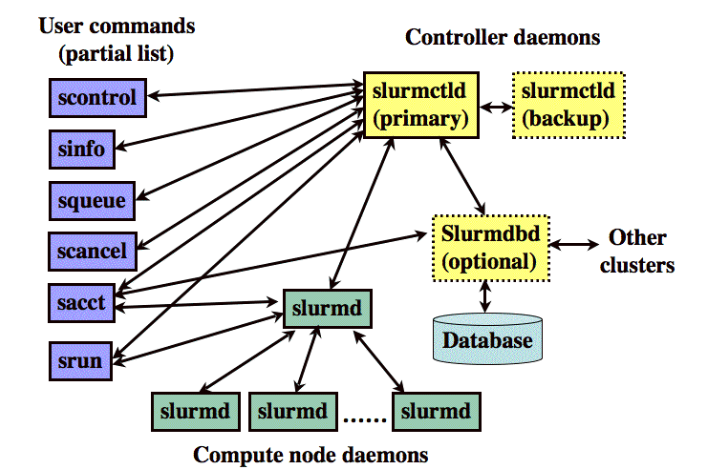
\includegraphics[width=0.8\textwidth]{slurm.png}
    \caption{Configuración SLURM \cite{fig4}}
    \label{fig:etiqueta}
  \end{figure}

  Algunas de las razones por las que se escoge Slurm para la gestión de recursos son:\cite{RHEL-SLURM-1}


  \begin{enumerate}
    \item Escalabilidad: Slurm es altamente escalable y puede manejar
          eficientemente grandes cargas de trabajo y múltiples usuarios en entornos de
          computación de alto rendimiento.
    \item Flexibilidad: Slurm es altamente configurable y permite a los
          usuarios definir y personalizar políticas de gestión de recursos, tales como
          prioridades de trabajos, particiones de clusters, políticas de colas, etc. Esto
          permite que Slurm se adapte a las necesidades específicas de cada grupo.
    \item Eficiencia: Slurm está diseñado para minimizar la sobrecarga del
          sistema y maximizar la eficiencia del uso de los recursos. Esto se logra
          mediante el uso de técnicas avanzadas de planificación y asignación de
          recursos, lo que garantiza que los trabajos se ejecuten de la manera más
          eficiente posible.
    \item Soporte de múltiples arquitecturas: Slurm soporta una amplia
          variedad de arquitecturas de hardware, incluyendo x86, ARM, IBM Power y otras
          arquitecturas de procesador.
    \item Comunidad activa: Slurm es un proyecto de código abierto con una
          comunidad de usuarios y desarrolladores activa y comprometida. Esto significa
          que hay una gran cantidad de recursos y soporte disponible en línea para ayudar
          a los usuarios de Slurm.
  \end{enumerate}

  Se anticipa que la implementación y utilización de Slurm resultará ser
  menos compleja que la de HTCondor, lo que confiere una mayor accesibilidad a la
  comunidad universitaria.

  \textbf{Jupyterhub}

  En el marco de este proyecto, se ha contemplado la utilización de JupyterHub como plataforma de acceso a los recursos computacionales, lo que permitirá a los usuarios disfrutar de una interfaz sencilla, centralizada y automatizada.

  JupyterHub es una plataforma sumamente versátil que se presta de manera excepcional para la gestión y ejecución simultánea de diversas instancias de Jupyter Notebook. Esta herramienta, por tanto, representa una alternativa idónea para contextos educativos o de investigación en los que varios usuarios necesitan emplear Jupyter Notebook de forma paralela.

  \begin{figure}[h]
    \centering
    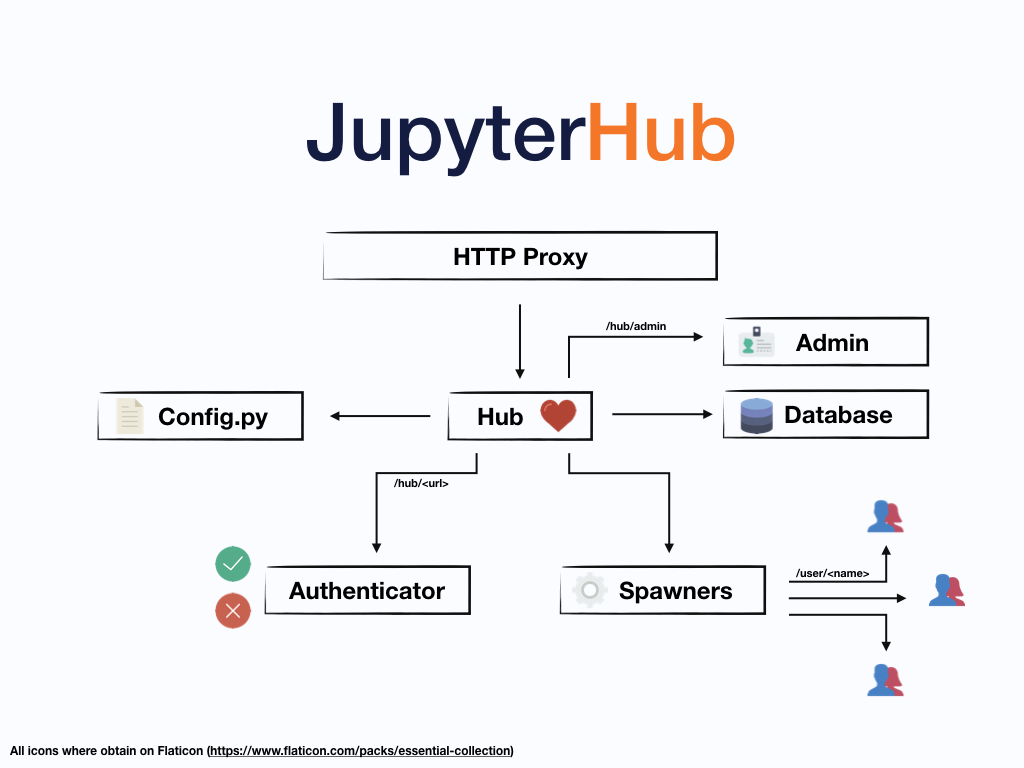
\includegraphics[width=0.7\textwidth]{hub.jpeg}
    \caption{Arquitectura JupyterHub \cite{fig5}}
    \label{fig:etiqueta}
  \end{figure}

  Al ejecutarse a través de un servidor central, el software de JupyterHub permite a los usuarios iniciar y detener sus sesiones de Jupyter Notebook de manera independiente. De esta manera, cada usuario dispone de su propio espacio de trabajo seguro y aislado en el que puede generar, llevar a cabo y compartir sus cuadernos de Jupyter, al tiempo que ofrece a los administradores de sistema un control riguroso del acceso y la seguridad de las múltiples instancias que se ejecutan.

  Con Slurm y JupyterHub, los usuarios del clúster podrán aprovechar al máximo los recursos disponibles y trabajar de manera más eficiente y colaborativa.
  \begin{tightcenter}
  \end{tightcenter}
\end{spacing}
\begin{spacing}{1.5}
  \begin{tightcenter}
    \section{4. Implementación y pruebas}
    \mylinespacing
  \end{tightcenter}

  \subsection{4.1 Implementando tecnologías}

  \textbf{Procedimiento}

  \textbf{Anexo No.1: Instalación y configuración de los computadores de la
    sala
    de cómputo}

  En este documento se registra el proceso de instalación y configuración de
  los
  computadores de la sala de cómputo de Jürgen Tischer, Departamento de
  Matemáticas, Universidad del Valle, Cali, Colombia. Además, se detallan las
  herramientas disponibles y su utilidad.

  El documento completo de instalación y configuración se encuentra en la
  sección
  de Anexos

  \subsection{4.2 Pruebas de control}

  En el proceso de verificar el correcto funcionamiento de los computadores y las integraciones, se emplean diversas herramientas, como las presentadas a continuación.

  \subsubsection {4.2.1 Comprobar conectividad básica con pdsh}

  El comando \code{alias} se configuró para verificar el estado de los equipos
  en
  el clúster. Este comando permite lanzar un comando de manera más sencilla,
  por
  ejemplo, \code{pdsh xeon "hostname"}, que devuelve el nombre de
  todos los
  equipos encendidos y conectados correctamente por ssh. Además, si se utiliza
  el
  argumento \code{uptime} en vez de \code{hostname}, se puede obtener más
  información sobre el estado de cada nodo.

  El resultado se ve de esta forma :

  \definecolor{codebackground}{RGB}{240,240,240}
  % Color de fondo del código
  \definecolor{codecomment}{RGB}{100,100,100}
  % Color de los comentarios
  \definecolor{codekeyword}{RGB}{0,0,255}
  % Color de las palabras clave
  \definecolor{codestring}{RGB}{163,21,21}
  % Color de las cadenas de texto

  \lstset{
    backgroundcolor=\color{codebackground},
    commentstyle=\color{codecomment},
    keywordstyle=\color{codekeyword},
    stringstyle=\color{codestring},
    basicstyle=\footnotesize\ttfamily,
    breakatwhitespace=false,
    breaklines=true,
    captionpos=b,
    frame=single,
    numberstyle=\tiny\color{codecomment},
    showspaces=false,
    showstringspaces=false,
    showtabs=false,
    tabsize=2,
    rulecolor=\color{codebackground}
  }
  \begin{lstlisting}[language=C]
      $ xeon "hostname"
      C4: C4
      E3: E3
      A2: A2
      ...
      B5: B5
  \end{lstlisting}

  \subsubsection {4.2.2 Comprobar funcionamiento en Mathematica}

  En Mathematica es fácil comprobar que la configuración paralela funciona
  correctamente. Para hacerlo, seleccione una configuración sencilla que
  incluya
  todos los nodos que desea utilizar. En nuestro caso, configuramos Lightweight
  Grid en las opciones de configuración paralela del kernel, con un kernel
  disponible para cada nodo. También es necesario desactivar
  \textit{RemoteKernel
    Objects}, que es un configurador automático que, por defecto, solo usa los
  kernels locales e ignora toda la configuración que se le coloca. Los kernels
  configurados se muestran en la Figura \ref{fig:etiqueta1}.  \newline  \newline

  \begin{figure}[h]
    \centering
    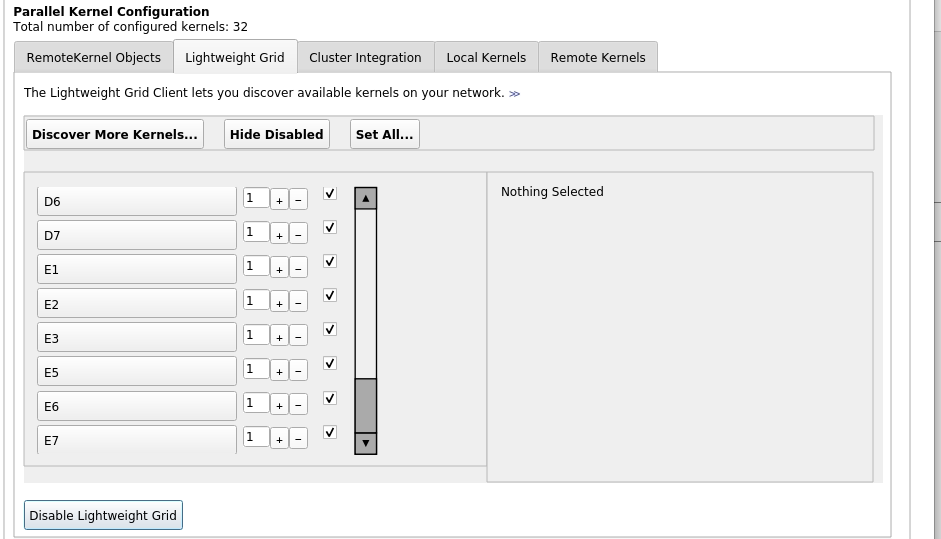
\includegraphics[width=0.9\textwidth]{mat.png}
    \caption{Configuración paralela en Mathematica}
    \label{fig:etiqueta1}
  \end{figure}

  Una vez que se haya completado esta configuración, podrás abrir un nuevo
  cuaderno (notebook) y escribir la siguiente instrucción: \code{LaunchKernels[
      ]}. De esta manera, la aplicación tratará de conectarse con los kernels
  configurados en cada nodo, tal como se muestra en la Figura
  \ref{fig:etiqueta2}

  \begin{figure}[h]
    \centering
    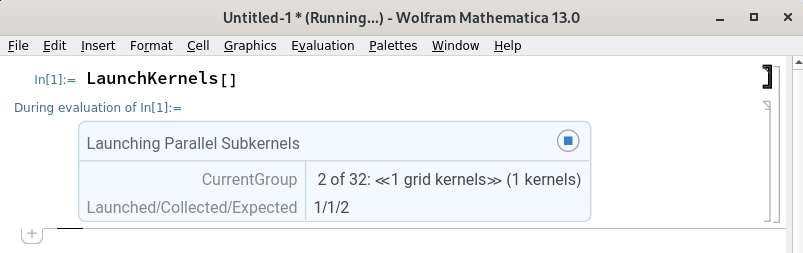
\includegraphics[width=0.9\textwidth]{mat1.png}
    \caption{Conexión de kernels y nodos}
    \label{fig:etiqueta2}
  \end{figure}

  En caso de que todo salga bien, se muestra una lista con todos los kernels
  iniciados, como se indica en la Figura \ref{fig:etiqueta3}

  \begin{figure}[h]
    \centering
    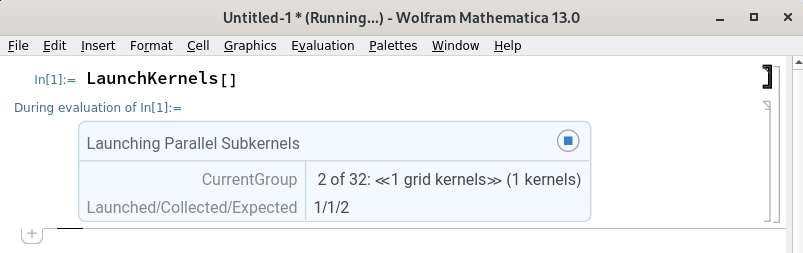
\includegraphics[width=0.9\textwidth]{mat4.png}
    \caption{Kenerls iniciados}
    \label{fig:etiqueta3}
  \end{figure}

  Si hay un error, Mathematica lo señalará. Normalmente el error incluirá
  información sobre el nodo que presenta problemas, así como una breve
  descripción del problema y posibles soluciones a aplicar, en la Figura
  \ref{fig:etiqueta4} se puede observa un error en Mathematica.

  \begin{figure}[h]
    \centering
    
\includegraphics[width=0.9\textwidth]{mat3.png}
    \caption{Información de error}
    \label{fig:etiqueta4}
  \end{figure}

  \subsubsection {4.2.3 Comprobar funcionamiento en Slurm}

  En Slurm, hay varios comandos básicos que nos permiten ver información sobre
  el
  estado de los nodos configurados.

  \begin{itemize}
    \item \textbf{sinfo}: Muestra el estado de los nodos. Es la primera
          herramienta que se debe utilizar para visualizar si hay algún
          problema de
          comunicación con los nodos.
    \item \textbf{srun}: Agrega una tarea a la cola de manera activa.
    \item \textbf{squeue}: Muestra la lista de tareas en cola, tanto pendientes
          como en ejecución.
    \item \textbf{scancel}: Cancela una tarea que se encuentra en la cola.
    \item \textbf{scontrol}: Se utiliza principalmente para cambiar el estado
          de los nodos.
  \end{itemize}

  Es posible probar rápidamente el funcionamiento de los nodos con \code{srun},
  de manera similar a como se utilizaba \code{pdsh}. En este caso, el comando
  utilizado es \code{srun -N10 hostname}. Esto solicitará a 10 nodos
  disponibles
  que ejecuten el comando \code{hostname}, devolviendo sus nombres. Si se
  utiliza
  el número total de nodos y todos devuelven su nombre, entonces la
  comunicación
  básica funciona. Sin embargo, solo esta prueba no es suficiente para
  determinar
  un problema de sincronización, ya que puede haber un problema en la
  comunicación del número de nodos en la tarea, donde cada nodo cree que es el
  único que ejecuta la tarea y no se da cuenta de que hay otros.

  \textbf{Helloworld Paralelo con C y C++}

  Para verificar la comunicación completa, se utilizó el programa de ``hola
  mundo''
  en paralelo con MPI, escrito en C. Esto se basa en el tutorial de
  mpitutorial.com \cite{HelloC}:

  \definecolor{codebackground}{RGB}{240,240,240}
  % Color de fondo del código
  \definecolor{codecomment}{RGB}{100,100,100}
  % Color de los comentarios
  \definecolor{codekeyword}{RGB}{0,0,255}
  % Color de las palabras clave
  \definecolor{codestring}{RGB}{163,21,21}
  % Color de las cadenas de texto

  \lstset{
    backgroundcolor=\color{codebackground},
    commentstyle=\color{codecomment},
    keywordstyle=\color{codekeyword},
    stringstyle=\color{codestring},
    basicstyle=\footnotesize\ttfamily,
    breakatwhitespace=false,
    breaklines=true,
    captionpos=b,
    frame=single,
    numberstyle=\tiny\color{codecomment},
    showspaces=false,
    showstringspaces=false,
    showtabs=false,
    tabsize=2,
    rulecolor=\color{codebackground}
  }

  \begin{lstlisting}[language=C]
    #include <stdio.h>
    #include <unistd.h>
    #include <mpi.h>
    
    int main(int argc, char** argv)
    {
      // Init the MPI environment
      MPI_Init(NULL, NULL);
      // Get the number of processes
      int world_size;
      MPI_Comm_size(MPI_COMM_WORLD, &world_size);
      // Get the rank of the process
      int world_rank;
      MPI_Comm_rank(MPI_COMM_WORLD, &world_rank);
      // Get the name of the processor
      char processor_name[MPI_MAX_PROCESSOR_NAME];
      int name_len;
      MPI_Get_processor_name(processor_name, &name_len);
      // Print a hello world message
      printf("Hello, World! from node %s, rank %d out of %d processors\n",
             processor_name, world_rank + 1, world_size);
      // Finalize the MPI environment
      MPI_Finalize();
    }
    \end{lstlisting}

  Para compilar este código es necesario contar con mpicc. Para hacerlo, se
  debe utilizar el siguiente comando: \code{mpicc c-mpi-hello.c -o
    c-mpi-hello}.

  Luego, el archivo debe ser accesible desde todas las máquinas en la misma
  ubicación. Para lograr esto, se utilizó un NFS, tal como se indica en la guía
  adjunta en el apartado NFS.

  Para ejecutar el código, se debe utilizar el comando \code{srun -N10
    /nfs/c-mpi-hello}.Esto asignará 10 nodos, cada uno con un hilo de proceso. El resultado tiene el siguiente formato :

    \begin{lstlisting}[language=C]
      $ srun -N4 c-mpi-hello
      Hello, World! from node bochica2, rank 2 out of 4 processors
      Hello, World! from node bochica3, rank 3 out of 4 processors
      Hello, World! from node bochica1, rank 1 out of 4     processors
      Hello, World! from node bochica4, rank 4 out of 4 processors
    \end{lstlisting}

  \textbf{Helloworld Paralelo con Python}

  Se puede lograr lo mismo utilizando Python. Se recomienda preparar un
  entorno utilizando conda o mamba en el NFS para que esté disponible para
  todos
  los nodos involucrados. Además, el entorno debe contener el paquete
  \code{mpi4py}. En nuestro caso, utilizamos la implementación de \code{mpich}.
  El entorno fue creado con el comando \code{conda create -p /nfs/anaconda
    anaconda mpi4py mpich}.

    En el siguiente código se muestra un programa en Python utilizando mpi4py para imprimir Hello World

    \begin{lstlisting}[language=python]
      # py-mpi-hello.py
      """
      Parallel Hello World
      """

      from mpi4py import MPI
      import sys
      import getpass

      size = MPI.COMM_WORLD.Get_size()
      rank = MPI.COMM_WORLD.Get_rank()
      name = MPI.Get_processor_name()
      user = getpass.getuser()

      sys.stdout.write(
      "%s: Hello, World! I am process %d of %d on %s.\n"
      % (user, rank+1, size, name))

    \end{lstlisting}
      
    Para activar el entorno de conda durante la ejecución de cada nodo, es más conveniente utilizar un archivo de sbatch que directamente con srun como se muestra a continuación:

    \begin{lstlisting}[language=python]
      # py-mpi-hello.sbatch
      #!/bin/sh
      #SBATCH -o /nfs/sbatch-examples/helloworld/py-mpi-hello.out
      #SBATCH --nodes=4
      #SBATCH --ntasks-per-node=1

      # Load conda commands from local installation
      source /opt/conda/etc/profile.d/conda.sh

      # Activate shared conda on nfs
      conda activate /nfs/conda

      # Run mpi example
      srun python /nfs/sbatch-examples/helloworld/py-mpi-hello.py
    \end{lstlisting}

    Utilizamos \code{sbatch py-mpi-hello.sbatch} para ejecutar la prueba y verificar su funcionamiento. El resultado debe ser como se muestra a continuación:

      \begin{lstlisting}[language=python]
      estudiante: Hello, World! I am process 2 of 4 on bochica2.
      estudiante: Hello, World! I am process 3 of 4 on bochica3.
      estudiante: Hello, World! I am process 4 of 4 on bochica4.
      estudiante: Hello, World! I am process 1 of 4 on bochica1. 
      \end{lstlisting}
      
  \subsection{4.3 Pruebas de eficiencia}  \label{chap:4.3}

  Se prepararon y realizaron dos pruebas para medir la eficiencia de los sistemas implementados.

      \textbf{Prueba de gridMathematica}

      Para probar el rendimiento en singular, multi-proceso y multi-máquina utilizamos el código de uno de los proyectos que se beneficiaron con la implementación de esta tesis (ver Capítulo 5, Influencia en proyectos destacados, para más detalles).

      De este código nos interesaremos por una parte en particular en donde existe una variable de puntos que afectan a un problema lineal, el cual resulta óptimo para probar el rendimiento de los sistemas.

      Preprint del proyecto mencionado y código de GitHub a utilizar. \cite{preprint} \cite{git}

      En los resultados mostrados solo se considera el tiempo de ejecución del cálculo realizado, no se toma en cuenta el tiempo que tarda en conectar los nodos ni en preparar las variables.

      Para las pruebas utilizamos diferentes escenarios, un DELL PRECISION T3610 equipado con Intel Xeon E5-1620 v2 @ 3.9GHz (4 núcleos físicos, 8 hilos de ejecución), lo comparamos con un HP Z1 equipado con un Intel i9-10900 @ 5.2 GHz para ver la diferencia de velocidad al escalar verticalmente una máquina y luego con el mismo Intel Xeon pero con 10 de esos.

      \textbf{Resultados Mathematica}

      Procesadores utilizados : 

      Xeon = Xeon E5-1620 v2 @ 3.9GHz 

      i9 = Intel i9-10900 @ 5.2 GHz

      \begin{figure}[h]
            \centering
            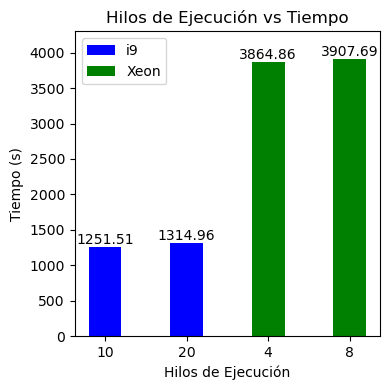
\includegraphics[width=0.5\textwidth]{tab1.png}
            \caption{Resultados Mathematica}
            \label{fig:etiqueta}
          \end{figure}

      En la figura 10 del anexo 2 podemos observar

      n=500

      \begin{figure}[h]
            \centering
            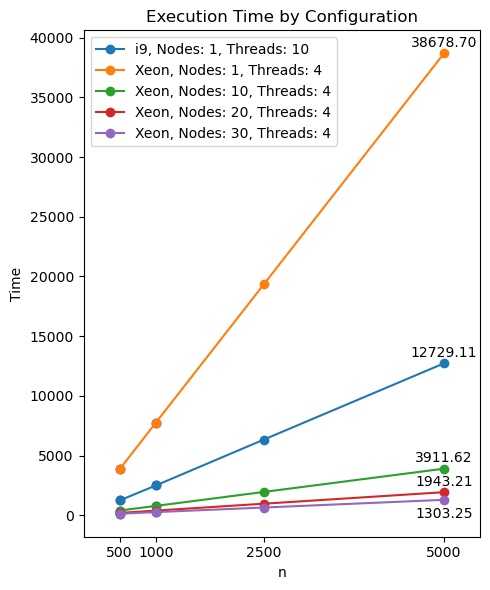
\includegraphics[width=0.5\textwidth]{tab2.png}
            \caption{Resultados Mathematica}
            \label{fig:etiqueta}
      \end{figure}

      En la siguiente gráfica se muestra la mejora porcentual en la eficiencia de generación de puntos por segundo.

      \begin{figure}[h]
            \centering
            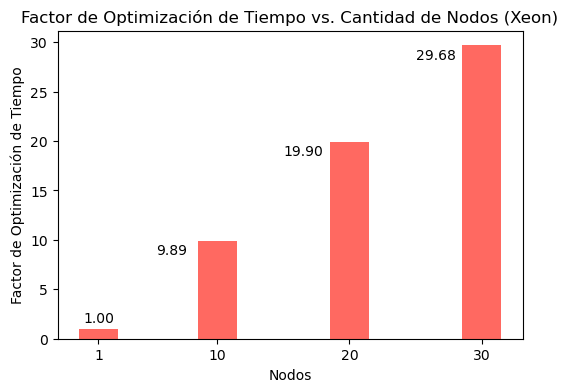
\includegraphics[width=0.5\textwidth]{tab3.png}
            \caption{Resultados Mathematica}
            \label{fig:etiqueta}
      \end{figure}

\textbf{Slurm - The Linpack Benchmark para sistemas distribuidos}

El benchmark Linpack es una prueba de rendimiento computacional que mide la capacidad de cálculo y eficiencia de un sistema informático en términos de velocidad y procesamiento numérico. Fue diseñado por Jack Dongarra en los años 70 en el Laboratorio Nacional de Oak Ridge, y se ha convertido en un estándar en el campo de la supercomputación y el rendimiento de los sistemas informáticos. Esta prueba utiliza la resolución de un sistema complejo de ecuaciones lineales como criterio. \cite{linpack}, \cite{hpl-linpack}, \cite{faq-linpack}

Con esta prueba, es posible evaluar el rendimiento y la capacidad de procesamiento de diferentes configuraciones computacionales y compararlos. En este proyecto, se utilizó Slurm para ejecutar la prueba en sistemas distribuidos. Se realizaron pruebas en diferentes configuraciones de nodos y núcleos por nodo, lo que permitió medir la eficiencia y el rendimiento en distintos escenarios. Los resultados se registraron para una evaluación detallada.

Para configurar adecuadamente la prueba, se utilizó una herramienta web que sugiere una configuración según la cantidad de nodos, la cantidad de tareas por nodo y la cantidad de memoria. \cite{tune-hpl-dat-file}

Durante la realización de esta investigación, se presentaron circunstancias imprevistas que afectaron el desarrollo de las pruebas de rendimiento en el entorno del clúster Bochica. Se detectaron problemas de mantenimiento en dicho entorno que comprometían su disponibilidad y estabilidad, poniendo en riesgo la precisión y confiabilidad de los resultados obtenidos.

En vista de esta situación, se tomó la decisión de replicar el entorno de slurm utilizando los 30 computadores Xeon E5-1620 v2 de la sala, mismos computadores de la prueba de Mathematica, en donde se procedió a ejecutar las pruebas de rendimiento. Aunque esta medida no estaba contemplada originalmente en el plan de investigación, se consideró como la mejor alternativa disponible para asegurar la integridad de las pruebas y la obtención de resultados fiables.

Cabe destacar que se tomaron todas las medidas necesarias para garantizar que el entorno secundario contara con una configuración similar al entorno Bochica, asimismo se minimizaron las diferencias de entorno a fin de mantener la consistencia en las pruebas realizadas.

\textbf{Resultados Slurm}

\begin{figure}[h]
      \centering
      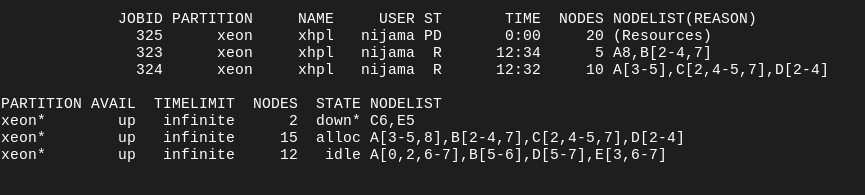
\includegraphics[width=0.5\textwidth]{a.png}
      \caption{Resultados Slurm}
      \label{fig:etiqueta}
\end{figure}

En el contexto del benchmark LINPACK, los datos obtenidos describen los resultados de ejecutar el benchmark en diferentes configuraciones de nodos y tareas por nodo.

\begin{itemize}
      \item "Nodos": representa el número de nodos utilizados en la ejecución del benchmark.
      \item "Tareas por nodo": indica el número de tareas (hilos de ejecución) asignadas a cada nodo.
      \item "Tiempo": es el tiempo en segundos que tardó el sistema en ejecutar el benchmark LINPACK en la configuración dada.
      \item "Gflops": representa el rendimiento medido en giga operaciones de punto flotante por segundo (GFLOPS) alcanzado durante la ejecución del benchmark.
\end{itemize}

En general, estos datos proporcionan una idea de cómo el rendimiento del sistema varía con respecto al número de nodos y tareas por nodo. A medida que se agregan más nodos y tareas, en general, el rendimiento mejora, aunque no de manera lineal debido a la comunicación y la sobrecarga asociadas con la coordinación entre nodos.

  \subsection{4.4 Automatización - Facilitar el uso}   \label{chap:4.4}

  \subsubsection{4.4.1 Scripts}

  En el desarrollo de este proyecto, se llevaron a cabo diversos scripts de
  automatización que permiten realizar tareas de mantenimiento y configuración
  de
  manera más eficiente y sistemática. Estos scripts han sido diseñados para
  optimizar procesos específicos dentro del proyecto y su implementación ha
  permitido reducir el tiempo de ejecución de tareas repetitivas y mejorar la
  calidad del trabajo.

  Estas son las funciones principales de los scripts de automatización:

  \begin{itemize}
    \item Encendido y apagado de computadores.
    \item Verificación del estado de los computadores y servicios.
    \item Actualización de software.
    \item Instalación de paquetes de software.
    \item Configuración completa de un nuevo equipo recién instalado o de
          un equipo antiguo formateado.
  \end{itemize}

  Esto permitirá minimizar las tareas comunes y de mantenimiento requeridas
  con menor esfuerzo. Además, estos scripts son altamente escalables y pueden
  ser
  adaptados para su uso en proyectos futuros, lo que representa una inversión a
  largo plazo en la mejora de la eficiencia y la calidad del trabajo.\cite{github}

  \subsection{4.5 Problemas encontrados}
  En el desarrollo de este proyecto, se presentaron problemas tanto previstos
  como inesperados, los cuales serán mencionados a continuación.

  \subsubsection{4.5.1 Problemas esperados}

  \begin{enumerate}
    \item \textbf{Heterogeneidad de los recursos computacionales:} El clúster
          Bochica y la sala de computación Jürgen Tischer contienen una
          variedad de
          recursos computacionales, incluyendo diferentes tipos de
          computadoras, sistemas
          operativos y versiones de software. Esto puede dificultar la
          optimización del
          sistema distribuido diseñado y requerir una mayor planificación y
          flexibilidad
          en el diseño y la implementación.
    \item \textbf{Antigüedad de los computadores:} Algunos de los computadores
          en el clúster Bochica y la sala de computación Jürgen Tischer son
          antiguos y
          pueden tener un impacto en la eficiencia y la capacidad de ejecutar
          tareas de
          investigación de manera óptima.
    \item \textbf{Dificultades en la adaptación a las nuevas herramientas:} La
          implementación de nuevas herramientas y tecnologías puede requerir un
          período
          de adaptación y aprendizaje para los usuarios, lo que puede retrasar
          los
          procesos de investigación y enseñanza. Además, pueden surgir
          problemas técnicos
          durante la instalación y configuración de las herramientas, lo que
          puede
          interferir en la eficiencia y productividad.
  \end{enumerate}

  \subsubsection{4.5.2 Problemas no esperados}

  \textbf{Problemas con el software}

  \begin{itemize}
    \item Problemas de licencias: Parte del software utilizado era
          propietario y resultó problematico el correcto uso de estas
          licencias,
          especialmente el software de Wolfram Mathematica.
  \end{itemize}

  \textbf{Problemas con el hardward}

  \begin{itemize}
    \item Cables mal acomodados: Los cables del clúster estaban mal
          acomodados, lo que generaba una dificultad para conocer las
          diferentes
          interconexiones entre los recursos.
    \item Cables faltantes: Se encontró que se requería un cable serial
          para la adecuada configuración de un switch que permite la
          interconexión entre
          los equipos del clúster.
    \item Permisos olvidados: Varios equipos del clúster debido a su
          desuso, se habían perdido las credenciales para utilizarlos de la
          manera
          adecuada
    \item Partes que requerían mantenimiento: Algunas partes del hardware
          requerían mantenimiento para su óptimo funcionamiento, pero esto no
          se había
          realizado.
    \item Desconocimiento de las limitaciones del hardware: Al principio no
          se conocían las limitaciones del hardware, lo que dificultaba su
          correcto uso y
          aprovechamiento.
    \item Hardware mal acomodado: El hardware estaba mal acomodado, lo que
          generaba problemas en la conexión y en el acceso a los recursos
          computacionales.
  \end{itemize}

  \textbf{Problemas con la Implementación del Sistema Distribuido}

  \begin{itemize}
    \item Falta de documentación clara para la implementación: La
          documentación para la implementación del sistema distribuido no era
          clara, lo
          que dificultaba su correcta implementación.
    \item Dificultades en la integración de los diferentes componentes del
          sistema: Se encontraron dificultades en la integración de los
          diferentes
          componentes del sistema distribuido, lo que limitaba su correcto
          funcionamiento.
    \item Limitaciones en la capacidad de paralelización: Se encontraron
          limitaciones en la capacidad de paralelización del sistema
          distribuido, lo que
          disminuía su eficiencia y efectividad.
  \end{itemize}

  \textbf{Problemas con las Herramientas Instaladas}

  \begin{itemize}
    \item Falta de compatibilidad con otras aplicaciones: Las herramientas
          instaladas no eran compatibles con otras aplicaciones, lo que
          limitaba su uso y
          efectividad.
    \item Dificultades en la configuración y uso: Se encontraron
          dificultades en la configuración y uso de las herramientas
          instaladas, lo que
          disminuía su efectividad.
    \item Falta de documentación y apoyo técnico: La falta de documentación
          y apoyo técnico para las herramientas instaladas limitaba su uso y
          efectividad.
  \end{itemize}

  \textbf{Problemas con las Pruebas de Rendimiento}

  \begin{itemize}
    \item Falta de recursos y tiempo para realizar las pruebas: No se
          contaba con los recursos y tiempo necesario para realizar las pruebas
          de
          rendimiento, lo que limitaba la evaluación de la infraestructura y
          las
          aplicaciones implementadas.
    \item Falta de una metodología clara para la realización de las
          pruebas: No había una metodología clara para la realización de las
          pruebas de
          rendimiento, lo que generaba incertidumbre en los resultados y
          dificultades en
          la interpretación de los mismos.
    \item Dificultades en la comparación de resultados con otras
          infraestructuras: Se encontraron dificultades en la comparación de
          los
          resultados obtenidos con otras infraestructuras similares, lo que
          disminuía la
          validez de los resultados.
    \item Falta de un sistema de seguimiento y monitoreo de las pruebas: No
          había un sistema de seguimiento y monitoreo de las pruebas, lo que
          dificultaba
          la identificación y solución de posibles problemas y limitaba la
          mejora
          continua de la infraestructura.
  \end{itemize}

  \mylinespacing
  \mylinespacing
  \begin{tightcenter}
  \end{tightcenter}
\end{spacing}
\begin{spacing}{1.5}
  \begin{tightcenter}
    \section{5. Influencia en Proyectos Destacados}
  \end{tightcenter}

  En este apartado queremos exponer algunos trabajos que se han visto
  beneficiados por el producto de esta tesis.

  \begin{enumerate}

    \item \textbf{Tesis de pregrado:} Dinámica del universo con Campos
          Taquiónicos. \newline
          \textbf{Datos de los investigadores:}
          \begin{itemize}
            \item Santiago Garcia Serna, estudiante de pregrado en Física
            \item Cesar Alonso Valenzuela Toledo, Ph.D. Profesor del
                  departamento de Física.
            \item Hernan Ocampo Duran, Ph.D. Profesor del departamento de
                  Física
          \end{itemize}
          \textbf{Departamento: } Física, Universidad del Valle \newline
          \textbf{Publicaciones asociadas al proyecto: } \newline Reconstructing
          the parameter space of non-analytical cosmological fixed points.\cite{Tesis1}

    \item \textbf{Nombre del proyecto:} Construcción numérica de datos
          iniciales en relatividad general. \newline
          \textbf{Datos de los investigadores:}
          \begin{itemize}
            \item Alejandro Estrada Llesta, estudiante de maestría en
                  matemáticas.
            \item Leon Escobar Diaz, Ph.D. Profesor del departamento de
                  Matemáticas.
          \end{itemize}
          \textbf{Departamento: } Matemáticas, Universidad del Valle. \newline
          \textbf{Publicaciones asociadas al proyecto: } \newline An hyperbolic
          approach for numerical constructing initial data sets of cosmological
          spacetimes. (En preparación)

    \item \textbf{Nombre del proyecto:} Exploración numérica de la ecuación
          de Benjamin-Ono en mallas no uniformes y con condiciones de frontera. \newline
          \textbf{Datos de los investigadores:} \newline
          Leon Escobar Diaz, Ph.D. Profesor del departamento de Matemáticas.
          \newline
          \textbf{Departamento: } Matemáticas, Universidad del Valle. \newline
          \textbf{Publicaciones asociadas al proyecto: } \begin{enumerate}
            \item A spectral-infinite element method for solving the hyperbolic
                  Einstein constraint equations. (En revisión)
            \item Numerical construction of asymptotically flat static
                  spacetimes from a Bartnik data set. (En progreso)
          \end{enumerate}

    \item \textbf{Nombre del proyecto:} Representación de enteros en
          sucesiones generalizadas de fibonacci y coordenadas de la ecuación de Pell.
          \newline
          \textbf{Datos de los investigadores:} \newline
          Carlos Alexis Gómez Ruiz, Ph.D. Profesor del departamento de
          Matemáticas. \newline
          \textbf{Departamento: } Matemáticas, Universidad del Valle. \newline
          \textbf{Publicaciones asociadas al proyecto: } \newline Por establecer.

    \item \textbf{Nombre del proyecto:} Aspectos numéricos y aplicaciones
          de matrices Toeplitz. \newline
          \textbf{Datos de los investigadores:} \newline
          Manuel Bogoya, Ph.D. Profesor del departamento de Matemáticas.\newline
          \textbf{Departamento: } Matemáticas, Universidad del Valle. \newline
          \textbf{Publicaciones asociadas al proyecto: } \newline Fast Toeplitz
          eigenvalue computations, joining interpolation-extrapolation matrix-less
          algorithms and simple-loop theory. \cite{Proy4}

    \item \textbf{Nombre del proyecto:} Simulación de micro-nadadores a
          través de métodos de elementos finitos acoplados a técnicas de aprendizaje de
          máquina. \newline
          \textbf{Datos de los investigadores:} \newline
          Stevens Paz, Ph.D. Profesor del departamento de Matemáticas. \newline
          \textbf{Departamento: } Matemáticas, Universidad del Valle. \newline
          \textbf{Publicaciones asociadas al proyecto: } \newline Chemoreception
          and chemotaxis of a three-sphere swimmer, (en revisión)\newpage

    \item \textbf{Nombre del proyecto:} Una variante del problema de Pillai en sucesiones recurrentes lineales. \newline
          \textbf{Datos de los investigadores:} \newline
          \begin{itemize}
            \item Carlos Alexis Gómez Ruiz, Ph.D. Profesor del departamento de Matemáticas.
            \item Jonathan García, estudiante de maestría en
                  matemáticas.
          \end{itemize}
          Carlos Alexis Gómez Ruiz, Ph.D. Profesor del departamento de Matemáticas. \newline
          \textbf{Departamento: } Matemáticas, Universidad del Valle. \newline
          \textbf{Publicaciones asociadas al proyecto: } \newline On a variant of Pillai problem: integers as difference between generalized Pell numbers and perfect powers \cite{Gomez2022}

  \end{enumerate}

  \mylinespacing
  \mylinespacing
  \begin{tightcenter}
  \end{tightcenter}
\end{spacing}
\begin{spacing}{1.5}
\begin{tightcenter}
\section{6. Trabajo Futuro}
\mylinespacing
\end{tightcenter}

\mylinespacing
\mylinespacing
\begin{tightcenter}
\end{tightcenter}
\end{spacing}

\begin{spacing}{1.5}
  \begin{tightcenter}
    \section{7. Discusión y conclusiones}
    \mylinespacing
  \end{tightcenter}

  A lo largo de este proyecto, se han obtenido logros sustanciales en relación con la implementación de un sistema distribuido destinado a la realización de investigaciones científicas en el Departamento de Matemáticas de la Universidad del Valle. Los resultados obtenidos demuestran la viabilidad de integrar diversas herramientas y tecnologías con el propósito de establecer un sistema eficiente y escalable que facilite la realización sistemática de investigaciones. 

Este servicio de computación paralela ha demostrado ser una herramienta efectiva para mejorar el procesamiento de datos en el ámbito académico. Adicionalmente, se han identificado oportunidades de mejora que contribuirán al incremento de la eficiencia, capacidad y facilidad de uso en un futuro. Aunque se presentaron algunos problemas durante el desarrollo del proyecto, estos fueron resueltos con éxito.

Durante el proceso de pruebas, hemos obtenido resultados que nos han dado una visión clara sobre el comportamiento esperado del sistema en diversas circunstancias. Además, los datos recopilados durante las pruebas permitieron obtener una mayor comprensión de las fortalezas y debilidades del sistema, lo que permitirá mejorar su rendimiento y eficacia en el futuro de manera significativa.

Este servicio representa un importante logro en el campo de la computación científica y tiene un impacto positivo en el desarrollo de la investigación en la Universidad del Valle y en la comunidad académica en general, ya que ha brindado a los investigadores de la Universidad del Valle una plataforma para llevar a cabo sus proyectos de investigación. La capacidad de paralelización ha permitido la ejecución simultánea de múltiples tareas, lo que ha acelerado los tiempos de procesamiento y ha aumentado la productividad en la obtención de resultados.

En términos generales, este proyecto ha establecido las bases necesarias para la implementación de sistemas distribuidos en la universidad, lo cual habilitará a estudiantes y docentes a aprovechar al máximo las capacidades de la computación distribuida con el fin de llevar a cabo investigaciones de mayor complejidad y sofisticación.

Finalmente, el objetivo principal de esta tesis, que era desarrollar un servicio de computación con capacidades de paralelización para la comunidad universitaria, no solo resultó siendo un proyecto completamente viable para la universidad, sino que se ha logrado con éxito. A través del aprovechamiento de los recursos existentes en el Departamento de Matemáticas de la Universidad del Valle, se ha creado un servicio que potencia el uso de los recursos informáticos mediante la paralelización.

  \mylinespacing
  \mylinespacing
  \begin{tightcenter}
  \end{tightcenter}
\end{spacing}
%% ref %%
\newpage
\section{8. referencias}
\printbibliography[heading=none]
%% ref %%
\begin{spacing}{1.5}
  \begin{tightcenter}
    \section{9. Anexos}
    \mylinespacing
  \end{tightcenter}

  \mylinespacing
  \mylinespacing
  \begin{tightcenter}
  \end{tightcenter}
\end{spacing}{1.5}


\end{document}